% Eight main slides for a 7--10 minute presentation; three backup slides.
\begin{frame}
  \textcolor{Teal}{\small AUFGABE 3 · CLUSTERING}
  \vspace{4mm}

  {\LARGE\bfseries Welche Cluster sind\par biologisch sinnvoll?}
  \vspace{2mm}

  {\large K-means, hierarchisches Clustering und Leiden}
  \vspace{7mm}

  \begin{columns}[T,onlytextwidth]
    \column{.31\textwidth}{\Huge\color{Teal}20.000}\par lebende PBMCs
    \column{.31\textwidth}{\Huge\color{Teal}37}\par biologische Marker
    \column{.31\textwidth}{\Huge\color{Teal}20}\par Spender · je 1.000 Zellen
  \end{columns}
  \vspace{5mm}
  \takeaway{Ein guter geometrischer Score ist noch kein Nachweis eines Zelltyps.}
  \source{Eigene Analyse: Notebook 03\_clustering, Lauf vom 07.09.2026. PBMC = mononukleäre Zellen des peripheren Bluts.}
\end{frame}

\begin{frame}{Gleiche Daten, drei Methodenfamilien}
  \begin{columns}[T,onlytextwidth]
    \column{.47\textwidth}
    \textbf{Vorverarbeitung}
    \begin{tikzpicture}[node distance=3mm,box/.style={draw=Line,fill=Pale,rounded corners=2pt,text width=5.7cm,align=center,minimum height=7mm,font=\small}]
      \node[box] (raw) {1.000 PBMCs je Spender, Seed 42};
      \node[box,below=of raw] (asinh) {$\operatorname{arcsinh}(x/5)$};
      \node[box,below=of asinh] (scale) {Z-Standardisierung je Marker};
      \node[box,below=of scale] (matrix) {$X$: 20.000 Zellen $\times$ 37 Marker};
      \draw[-{Stealth},Teal] (raw)--(asinh);
      \draw[-{Stealth},Teal] (asinh)--(scale);
      \draw[-{Stealth},Teal] (scale)--(matrix);
    \end{tikzpicture}
    \column{.49\textwidth}
    \textbf{44 Konfigurationen}
    \small
    \begin{itemize}
      \item K-means: 7 Werte für $k$, je 10 Starts.
      \item Hierarchisch: Single, Average, Complete und Ward; je 7 Werte für $k$.
      \item Leiden: 3 Nachbarzahlen $\times$ 3 Resolutionen; gewichteter Graph aus $X$.
    \end{itemize}
    \vspace{1mm}
    $k\in\{2,3,4,6,8,10,12\}$\par
    $n\in\{10,30,60\}$; $r\in\{0{,}3;0{,}7;1{,}2\}$
  \end{columns}
  \takeaway{Auswahl je Methode: kleinster Davies--Bouldin-Index unter den Lösungen mit Stabilität $\geq 0{,}6$.}
  \source{Stabilität: 10 Wiederholungen mit je 80\,\% der Zellen pro Spender; Skalierung und Clustering erneut fitten. Details in Reservefolie 10.}
\end{frame}

\begin{frame}{Die Auswahl liefert sehr unterschiedliche Lösungen}
  \small
  \renewcommand{\arraystretch}{1.3}
  \setlength{\tabcolsep}{5pt}
  \begin{tabular}{@{}llrrrr@{}}
\toprule
Methode & Parameter & Cluster & DB $\downarrow$ & Stabilität & Größtes Cluster\\
\midrule
K-means & $k=4$ & 4 & 2{,}363 & 0{,}995 & 37{,}780\,\% \\
Single & $k=2$ & 2 & 0{,}264 & 1{,}000 & 99{,}995\,\% \\
Average & $k=2$ & 2 & 0{,}894 & 0{,}602 & 99{,}975\,\% \\
Complete & $k=2$ & 2 & 0{,}948 & 0{,}617 & 99{,}960\,\% \\
Ward & $k=6$ & 6 & 2{,}522 & 0{,}611 & 38{,}220\,\% \\
Leiden & $n=30, r=1{,}2$ & 18 & 2{,}361 & 0{,}683 & 17{,}940\,\% \\
\bottomrule
\end{tabular}
\par
  \vspace{3mm}
  K-means und Leiden: ähnliche DB-Werte, unterschiedliche Auflösung und Stabilität.
  \takeaway{Clustergrößen mitlesen: Single, Average und Complete bündeln jeweils über 99,9\,\% der Zellen.}
  \source{DB = Davies--Bouldin-Index, kleiner ist besser. Stabilität = ungewichteter Mittelwert der Cluster-Median-Jaccards. Eigene Notebook-Ergebnisse.}
\end{frame}

\begin{frame}{Warum der beste DB-Wert hier täuscht}
  \begin{columns}[T,onlytextwidth]
    \column{.57\textwidth}
    \textbf{Single Linkage, $k=2$}
    \vspace{4mm}

    {\Huge\color{Teal}19.999}\quad Zellen in C0\par\vspace{3mm}
    {\Huge\color{Rust}1}\hspace{21mm} Zelle in C1
    \vspace{4mm}

    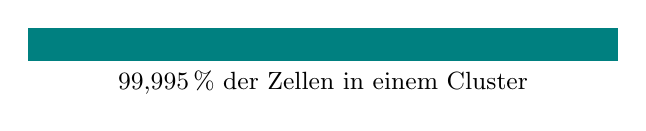
\begin{tikzpicture}
      \fill[Teal] (0,0) rectangle (7.5,.42);
      \node[below,font=\small,align=left] at (3.75,0) {99,995\,\% der Zellen in einem Cluster};
    \end{tikzpicture}
    \column{.39\textwidth}
    \begin{block}{Trotzdem ausgezeichnete Kennzahlen}
      DB: \textbf{0,264}\par
      Stabilität: \textbf{1,000}
    \end{block}
    \small
    Die Trennung eines isolierten Events kann geometrisch günstig und beim Resampling reproduzierbar sein.
  \end{columns}
  \vspace{3mm}
  \takeaway{Diese Lösung trennt hauptsächlich einen Ausreißer ab; sie beantwortet die Frage nach Zelltypen nicht.}
  \source{Balken zeigt den Anteil der großen Gruppe; die einzelne Zelle ist maßstabsgetreu nicht sichtbar. Eigene Ergebnisse; DB-Definition: scikit-learn.}
\end{frame}

\begin{frame}{K-means gruppiert grob, Leiden teilt feiner auf}
  \begin{columns}[T,onlytextwidth]
    \column{.49\textwidth}
    \textcolor{Teal}{\textbf{K-means · 4 Cluster}}
    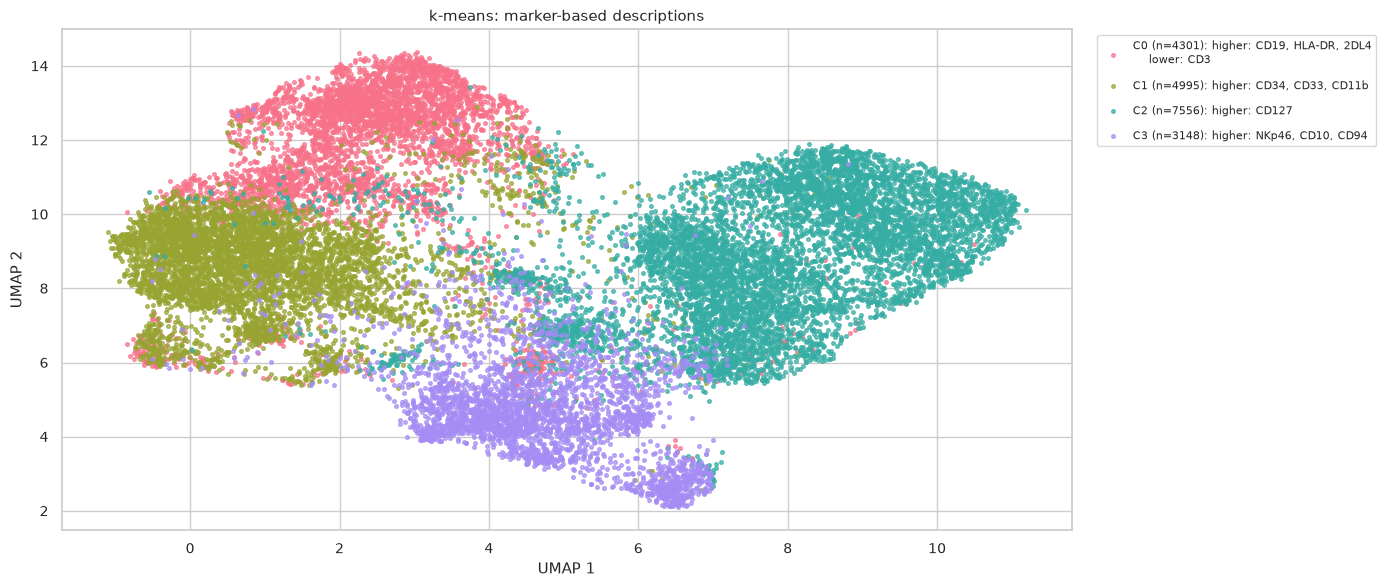
\includegraphics[width=\linewidth,height=33mm,keepaspectratio,trim=0 0 86mm 0,clip]{figures/umap_kmeans.png}
    \small 3.148--7.556 Zellen pro Cluster\par
    Mittlere Stabilität: \textbf{0,995}
    \column{.49\textwidth}
    \textcolor{Indigo}{\textbf{Leiden · 18 Cluster}}
    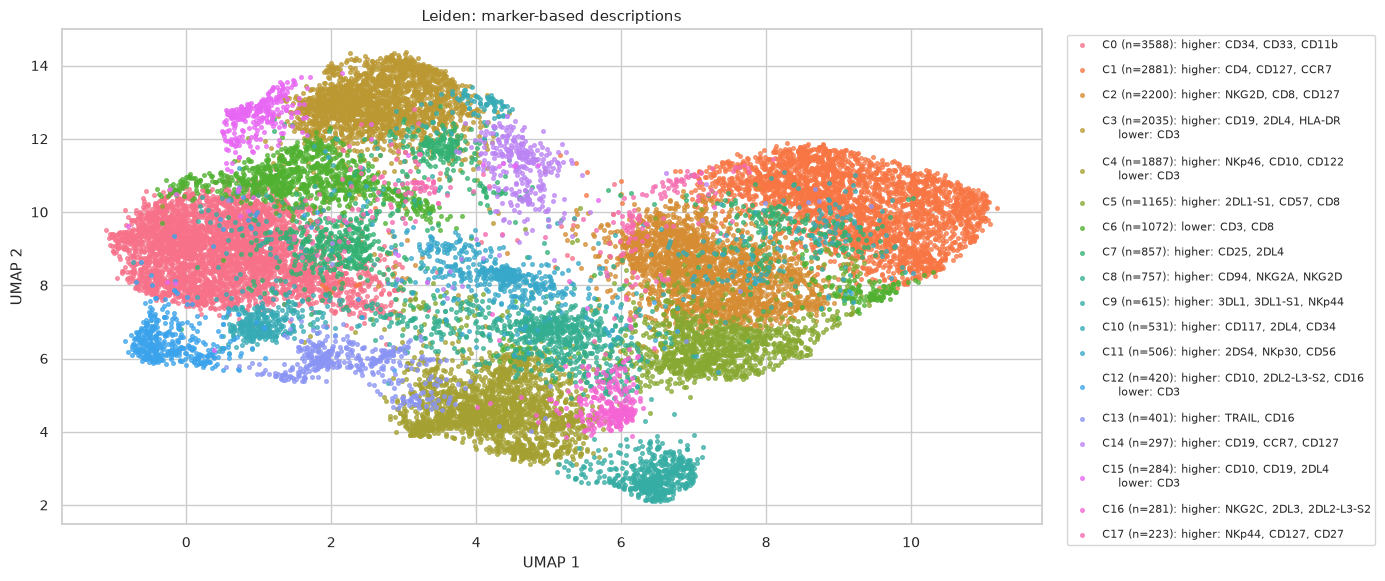
\includegraphics[width=\linewidth,height=33mm,keepaspectratio,trim=0 0 86mm 0,clip]{figures/umap_leiden.png}
    \small 223--3.588 Zellen pro Cluster\par
    Mittlere Stabilität: \textbf{0,683}
  \end{columns}
  \takeaway{Die feinere Aufteilung liefert Kandidaten für Untergruppen, deren Stabilität einzeln geprüft werden muss.}
  \source{Original-UMAPs aus dem Notebook, Legenden für die Gegenüberstellung ausgeblendet. Gleiche Einbettung; Farben sind je Methode lokal. Clustering und Scores verwenden alle 37 Marker, nicht UMAP.}
\end{frame}

\begin{frame}{Der Mittelwert verdeckt instabile Cluster}
  
\includegraphics[width=\textwidth]{figures/cluster_stability.pdf}
  \begin{columns}[T,onlytextwidth]
    \column{.48\textwidth}
    \small\textbf{Leiden: 4 von 18 unter 0,6}\par
    C15 und C16 liegen nur bei 0,111 und 0,120.
    \column{.48\textwidth}
    \small\textbf{Ward: 3 von 6 unter 0,6}\par
    Die Konfiguration bleibt mit Mittelwert 0,611 zugelassen.
  \end{columns}
  \takeaway{Die Grenze 0,6 gilt für den Mittelwert der Konfiguration, nicht für jeden einzelnen Cluster.}
  \source{Jeder Punkt: ein Cluster der ausgewählten Lösung. Gespeicherte Median-Jaccards; die gestrichelte Linie dient zum Vergleich der Einzelwerte.}
\end{frame}

\begin{frame}{Markerprofile liefern biologische Hypothesen}
  \small
  \renewcommand{\arraystretch}{1.35}
  \begin{tabular}{@{}>{\raggedright\arraybackslash}p{2.1cm}>{\raggedright\arraybackslash}p{3.4cm}>{\raggedright\arraybackslash}p{3.6cm}>{\raggedright\arraybackslash}p{3.6cm}@{}}
    \toprule
    Hypothese & K-means & Leiden & Einordnung\\
    \midrule
    B-Zell-artig & C0: CD19\up, HLA-DR\up, CD3\down & C3: CD19\up, HLA-DR\up, CD3\down & Ähnliche relative Profile\\
    NK-Zell-artig & C3: NKp46\up, CD94\up & C4: NKp46\up, CD122\up, CD3\down & Kandidaten; weitere Marker prüfen\\
    Unklar & C1: CD34\up, CD33\up; C2: CD127\up & Weitere Untergruppen & Profile reichen zur Zuordnung nicht aus\\
    \bottomrule
  \end{tabular}\par
  \vspace{1mm}
  \textbf{Pfeile beschreiben relative Cluster-Mediane.}\par
  Keine Positiv-/Negativ-Gates und kein Nachweis der Koexpression in einzelnen Zellen.
  \takeaway{Die Profile stützen Zelltyp-Hypothesen, ersetzen aber keine validierte Zuordnung.}
  \source{Eigene, vorläufige Interpretation der Notebook-Profile. Biologischer Kontext: Horowitz et al. (2013), doi:10.1126/scitranslmed.3006702. Ähnliche Profile belegen keine Übereinstimmung der Zellmengen.}
\end{frame}

\begin{frame}{Unsere Bewertung: robuste Grobstruktur, offene Zelltypen}
  \begin{columns}[T,onlytextwidth]
    \column{.48\textwidth}
    \begin{block}{K-means als grobe Ausgangslösung}
      Vier sehr stabile Gruppen; plausible Markerprofile für einen Teil der Cluster.
    \end{block}
    \begin{block}{Leiden für feinere Hypothesen}
      Mehr Untergruppen, darunter mehrere instabile Cluster. Kein pauschaler biologischer Vorteil.
    \end{block}
    \column{.48\textwidth}
    \textbf{Für die biologische Entscheidung}
    \small
    \begin{itemize}
      \item Markerkombinationen und Koexpression prüfen.
      \item Verteilung je Spender und Aufnahmetag kontrollieren.
      \item Neue Ausgangsstichproben untersuchen, besonders für kleine Gruppen.
    \end{itemize}
    \vspace{2mm}
    Single, Average und Complete sind in der ausgewählten Form stark degeneriert; Ward ist weniger stabil.
  \end{columns}
  \takeaway{Quantitative Bewertung und Markerinterpretation gemeinsam nutzen. Ein eindeutiger biologischer Sieger ist noch nicht belegt.}
  \source{Bewertung der ausgewählten Lösungen auf dieser Stichprobe; keine allgemeine Rangfolge der Algorithmen.}
\end{frame}

\appendix
\begin{frame}{Reserve: Was ändert sich gegenüber 200 Zellen je Spender?}
  \small
  \renewcommand{\arraystretch}{1.3}
  \begin{tabular}{@{}lll@{}}
    \toprule
    Methode & 200 Zellen/Spender & 1.000 Zellen/Spender\\
    \midrule
    K-means & $k=4$; Stabilität 0,973 & $k=4$; Stabilität 0,995\\
    Single / Average / Complete & jeweils $k=4$ & jeweils $k=2$\\
    Ward & keine zugelassene Konfiguration & $k=6$; Stabilität 0,611\\
    Leiden & $n=30$, $r=0{,}7$; 8 Cluster & $n=30$, $r=1{,}2$; 18 Cluster\\
    \bottomrule
  \end{tabular}\par
  \vspace{5mm}
  \textbf{Zwei Änderungen gleichzeitig:}
  \begin{itemize}
    \item Fünfmal so viele Zellen: 4.000 $\rightarrow$ 20.000 insgesamt.
    \item Zusätzlich $k=2$ und $k=3$ im Raster der distanzbasierten Verfahren.
  \end{itemize}
  \takeaway{Die Unterschiede können nicht allein der größeren Stichprobe zugeschrieben werden.}
  \source{200er-Referenz: geprüfter Neulauf mit Grenze 0,6, nicht die früheren veralteten Notebook-Ausgaben. Quellen: beide Untersuchungsberichte im Repository.}
\end{frame}

\begin{frame}{Reserve: Wie wird Stabilität berechnet?}
  \small
  Für Wiederholung $b$ werden dieselben behaltenen Zell-IDs $R_b$ verglichen:
  \[
    J_{c,b}=\max_j\frac{|(C_c\cap R_b)\cap D_{j,b}|}{|(C_c\cap R_b)\cup D_{j,b}|},
    \qquad S=\frac{1}{K}\sum_{c=1}^{K}\operatorname{median}_b J_{c,b}.
  \]
  $C_c$: ursprünglicher Cluster; $D_{j,b}$: neuer Cluster auf den behaltenen Zellen.
  \begin{itemize}
    \item 10 Wiederholungen, jeweils 80\,\% innerhalb jedes Spenders ohne Zurücklegen.
    \item Skalierung und Clustering neu fitten; Methodenparameter bleiben gleich.
    \item Abwesende Cluster: NaN. Mindestens 6 auswertbare Wiederholungen im aktuellen Lauf.
    \item Keine Mindestgröße; ein Singleton kann beim Behalten stabil sein.
  \end{itemize}
  \takeaway{Gemessen wird Robustheit innerhalb der Ausgangsstichprobe, nicht Übertragbarkeit auf neue Spender.}
  \source{Eigene Notebook-Implementierung; Referenzzuordnungen sind keine Ground Truth.}
\end{frame}

\begin{frame}{Reserve: Quellen und Reproduzierbarkeit}
  \footnotesize
  \textbf{Eigene Ergebnisse}\par
  \texttt{notebooks/03\_clustering.ipynb}, Lauf vom 07.09.2026.\par
  20.000 Zellen, Seed 42, Arcsinh-Cofaktor 5, Z-Standardisierung; 44 + 440 Fits.\par
  Tabellen und UMAPs direkt aus den gespeicherten Notebook-Ausgaben exportiert.
  \vspace{3mm}

  \textbf{Datensatz und biologischer Kontext}\par
  Horowitz et al. (2013). Genetic and environmental determinants of human NK cell diversity revealed by mass cytometry. \emph{Science Translational Medicine}.\par
  \href{https://doi.org/10.1126/scitranslmed.3006702}{doi:10.1126/scitranslmed.3006702}\par
  Arvaniti \& Claassen (2017). Sensitive detection of rare disease-associated cell subsets via representation learning. \emph{Nature Communications}.\par
  \href{https://doi.org/10.1038/ncomms14825}{doi:10.1038/ncomms14825}
  \vspace{3mm}

  \textbf{Methodendokumentation}\par
  \href{https://scikit-learn.org/stable/modules/clustering.html\#davies-bouldin-index}{scikit-learn: Davies--Bouldin-Index}\quad
  \href{https://docs.scipy.org/doc/scipy/reference/generated/scipy.cluster.hierarchy.linkage.html}{SciPy: Linkage}\quad
  \href{https://scanpy.readthedocs.io/en/stable/api/generated/scanpy.tl.leiden.html}{Scanpy: Leiden}
\end{frame}
